\begin{graphicspathcontext}{{./chapters/cps/imgs/},{./chapters/cps/imgs/auto/},\old}

\sidecite{Baheti2011CPSImpact}
\begin{frame}{The Conceptual Landscape}
	\begin{columns}
		\begin{column}{.5\linewidth}
			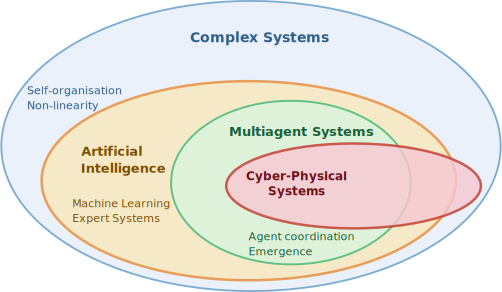
\includegraphics{cps_venn}
		\end{column}
		\begin{column}{.5\linewidth}
			\begin{description}
			\item[Complex Systems] provide the theoretical ground: emergence, self-organisation, non-linearity
			\item[Artifical Intelligence] provides the cognitive machinery: reasoning, learning, optimisation
			\item[Multiagent System] provides the architectural paradigm: decentralisation, coordination, autonomy
			\item[Cyber-Physical System] is the \emph{application domain} sitting at the intersection: it requires all three
			\end{description}
		\end{column}
	\end{columns}
\end{frame}

\sidecite{CossentinoGaudHilaireGallandKoukam2010_1}
\begin{frame}{Why MAS is the Right Model for CPS}
	\smaller
	\begin{columns}
		\begin{column}{.5\linewidth}
			\Emph{Mapping CPS requirements to MAS features:}
			\begin{stabularx}{X|X}
			\tabularhead{CPS Requirement}{MAS Answer} \\
			Distributed sensing      & Agent perception loop \\
			\hline
			Real-time reaction       & Reactive architecture \\
			\hline
			Goal-directed control    & BDI intentionality \\
			\hline
			Fault tolerance          & Agent redundancy \\
			\hline
			Openness                 & Dynamic agent population \\
			\hline
			Coordination             & Protocols \& contracts \\
			\hline
			Learning \& adaptation   & Reinforcement learning agents \\
			\end{stabularx}
		\end{column}
		\begin{column}{.5\linewidth}
			\begin{block}{Holonic MAS (HMAS)}
				Agents can be \emph{aggregated} into higher-level \Emph{holons}:
				\[
				h = (\{h_1, h_2, \dots, h_k\}, \{h_{k+1}, h_{k+2}, \dots, h_n\}, \dots)
				\]
				This naturally mirrors the \emph{hierarchical} layers of CPS
				(sensor $\rightarrow$ edge $\rightarrow$ cloud).
			\end{block}
			\begin{exampleblock}{SARL}
				The \emph{SARL} agent-oriented language provides:
				\begin{itemize}
				\item Capacities \& Skills
				\item Spaces \& Contexts
				\item Built-in BDI support
				\item Holonic agent model
				\end{itemize}
			\end{exampleblock}
		\end{column}
	\end{columns}
\end{frame}

\end{graphicspathcontext}

\endinput
